\chapter{Einleitung}

Sichtbarkeitsgraphen sind Graphen, die alle Knotenpaare miteinander verbinden, die sich \emph{sehen} können, auf deren \emph{Luftlinie} sich also keine \emph{Hindernisse} befinden.
Aus einer Küstenlinie kann ein Sichtbarkeitsgraph erstellt werden, indem die Knoten auf der Küstenlinie mit allen Knoten verbunden werden, deren Luftlinie keine Küste kreuzt.
\autoref{fig:thessaloniki-visibility} zeigt einen Ausschnitt eines solchen Sichtbarkeitsgraphen.
Zu sehen ist der Hafen der griechischen Stadt Thessaloniki.

Das Finden von kürzesten Pfaden ist in solchen Graphen rechenintensiver als etwa auf Straßengraphen mit vergleichbarer Knotenanzahl, da sie unter anderem einen höheren durchschnittlichen Knotengrad und keine inhärente hierarchische Struktur besitzen.
Zwar gibt es Möglichkeiten, den Graphen zu verändern, und schneller Pfade zwischen Knoten zu berechnen, etwa durch Triangulierung oder Rasterisierung, jedoch sind diese Pfade nicht mehr garantiert optimal.

Im Folgenden wird untersucht, inwiefern sich zwei Techniken zum schnellen Finden von kürzesten Pfaden und kürzesten Pfad-Distanzen (\emph{Contraction Hierarchies} und \emph{Hierarchical Hub Labeling}) auf diese Graphen anwenden lassen.

\begin{figure}[ht]%
  \centering
  \subfloat[\centering aegaeis-visibility]{{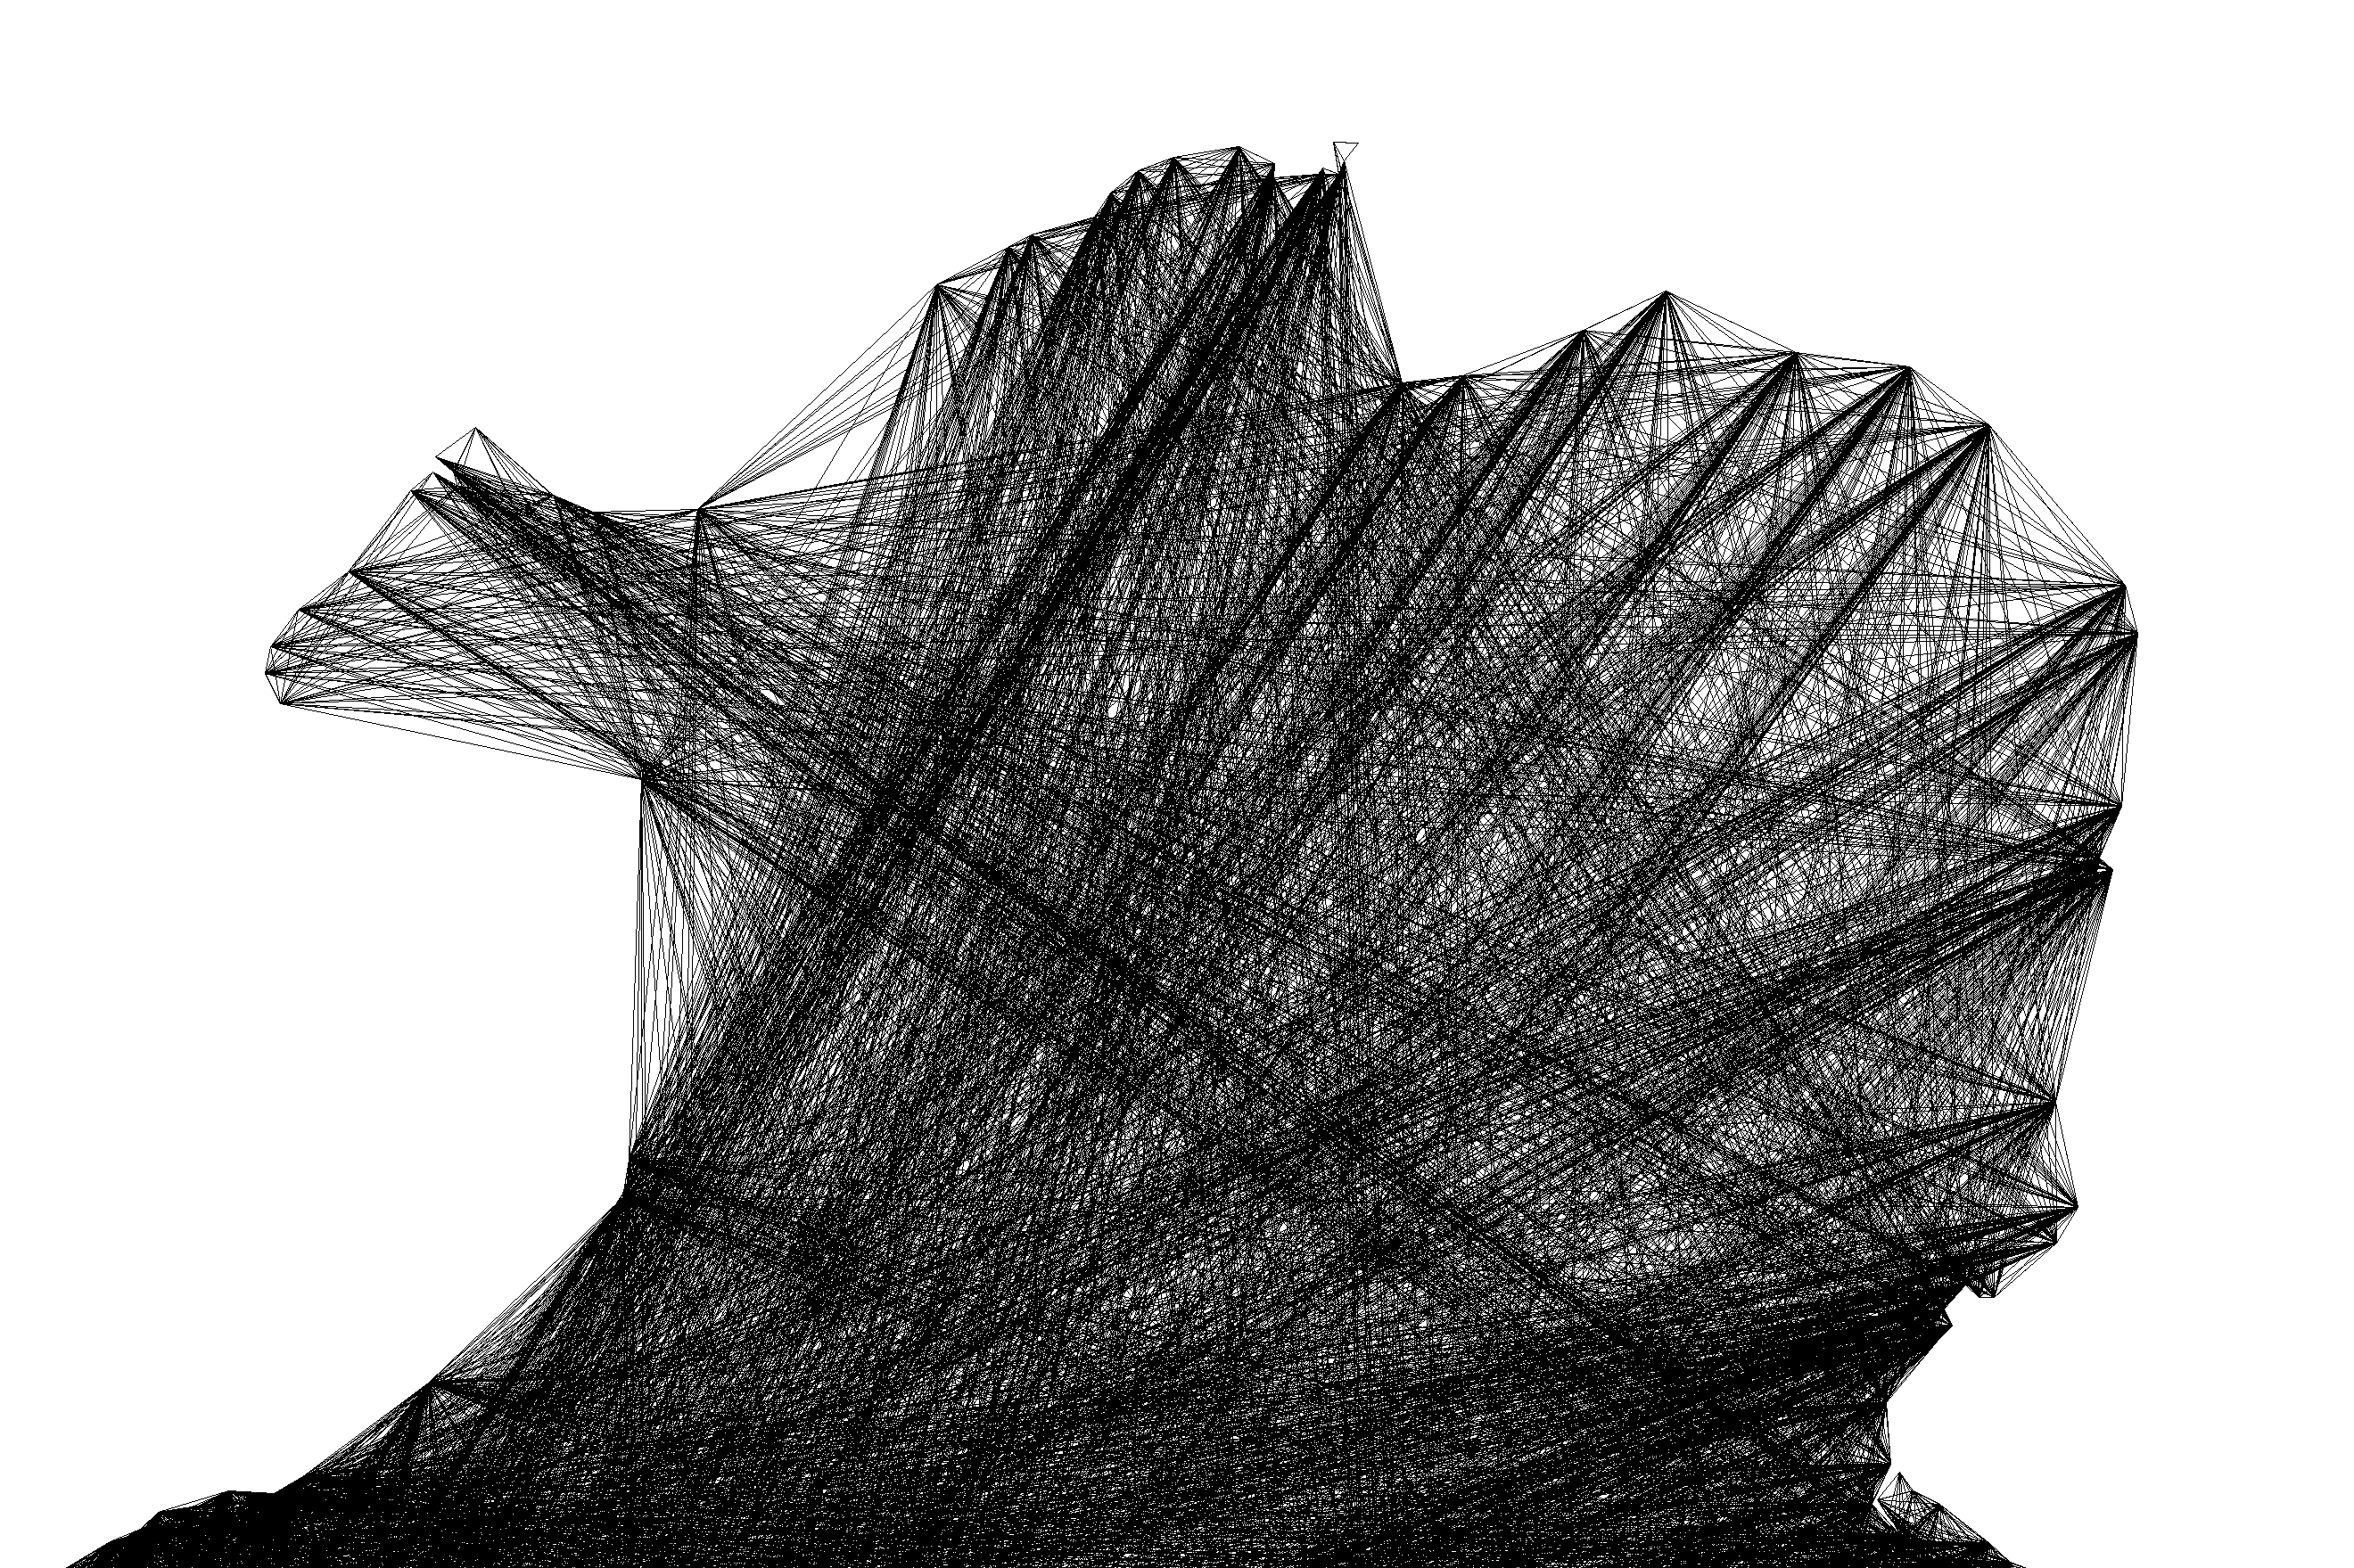
\includegraphics[width=.5\linewidth]{img/thessaloniki-visibility.png}}}%
  \caption{Sichtbarkeitsgraph des Hafens von Thessaloniki}%
  \label{fig:thessaloniki-visibility}%
\end{figure}
% 
% 
% 
% 
% \section{Speedup-Techniken}
% 
% Die betrachteten Speedup-Techniken zum Finden kürzester Pfade benötigen eine Phase der Vorbehandlung (\emph{preprocessing}), damit danach kürzeste Pfad Anfragen (\emph{queries}) schneller beantwortet werden können.
% Die für das Preprocessing benutzte Rechenzeit und der Memory-Overhead sollte dabei in einem sinnvollen Verhältnis zum Speedup und der Anzahl der Queries stehen.
% Ist der Speedup besonders hoch, so lohnt es sich mehr in das Preprocessing zu investieren.
% 
% \todo{Speedup Techniken auflisten, Aufwand / Benefit Diagram}
% 